\documentclass[conference]{IEEEtran}
\IEEEoverridecommandlockouts

\usepackage{cite}
\usepackage{amsmath,amssymb,amsfonts}
\usepackage{algorithm}
\usepackage{algpseudocode}
\usepackage{graphicx}
\usepackage{textcomp}
\usepackage{xcolor}
\usepackage{booktabs}
\usepackage{tikz}
\usetikzlibrary{shapes.geometric, arrows.meta, positioning, fit, backgrounds, calc}
\usepackage{url}
\usepackage{balance}
\def\BibTeX{{\rm B\kern-.05em{\sc i\kern-.025em b}\kern-.08em T\kern-.1667em\lower.7ex\hbox{E}\kern-.125emX}}

% ---------------------------------------------------------------
% TikZ styles (compact, conference-column friendly)
% ---------------------------------------------------------------
\tikzstyle{data} = [rectangle, rounded corners, minimum width=2.0cm, minimum height=0.6cm, text centered, draw=black, fill=blue!12, font=\scriptsize]
\tikzstyle{store} = [cylinder, shape border rotate=90, minimum width=1.7cm, minimum height=0.6cm, text centered, draw=black, fill=orange!15, font=\scriptsize]
\tikzstyle{proc} = [rectangle, rounded corners, minimum width=2.0cm, minimum height=0.6cm, text centered, draw=black, fill=green!12, font=\scriptsize]
\tikzstyle{ctrl} = [diamond, aspect=2, minimum width=1.4cm, text centered, draw=black, fill=red!10, font=\scriptsize, inner sep=1pt]
\tikzstyle{arr} = [-{Stealth[length=2mm]}, thick]
\tikzstyle{lab} = [font=\tiny, text=gray]

\begin{document}

\title{An Autonomous Financial Reasoning Agent over a Hybrid Knowledge-Graph and Vector Store: Architecture, Pipelines, and Empirical Evaluation}

\author{\IEEEauthorblockN{Abdul Basit}
\IEEEauthorblockA{\textit{Independent Research}\\
basitmal36@gmail.com}}

\maketitle

% =================================================================
\begin{abstract}
Large language models (LLMs) struggle with financial question answering when evidence is fragmented across structured tables, unstructured filings, and multilingual news. We present an \emph{agentic financial reasoning system} that couples a Neo4j knowledge graph and a Qdrant vector store with an OpenRouter-hosted LLM, orchestrated by a LangGraph state machine. The system implements a six-phase pipeline: document ingestion and entity resolution, hybrid retrieval (graph expansion + dense similarity with reciprocal-rank fusion), tool-augmented reasoning over retrieved context, validator--corrector quality gates, evidence-grounded report generation, and a persistent audit ledger for full traceability. A FastAPI gateway and Streamlit interface expose the pipeline interactively. We evaluate the system on a curated corpus of financial filings and news, measuring retrieval precision, answer faithfulness, and end-to-end latency. Empirical results show that hybrid graph--vector retrieval improves evidence precision by a large margin over dense-only baselines, while the validator--corrector loop measurably reduces hallucinated citations. All components are released as an open repository with a reproducible CI pipeline. The architecture is deliberately modular so that retrieval, reasoning, and governance layers can evolve independently.
\end{abstract}

\begin{IEEEkeywords}
financial NLP, retrieval-augmented generation, knowledge graphs, agentic systems, LangGraph, RAG, LLM evaluation
\end{IEEEkeywords}

% =================================================================
\section{Introduction}
\IEEEPARstart{A}{nswering} questions about companies, markets, and risk requires reasoning over \emph{heterogeneous} evidence: balance-sheet tables, filings, earnings-call transcripts, and time-sensitive news. Pure dense retrieval conflates entities (e.g., similarly named subsidiaries), while pure symbolic systems fail on free-text nuance. Retrieval-augmented generation (RAG) \cite{lewis2020rag} mitigates hallucination but, in its vanilla form, retrieves flat chunks without relational structure.

This paper describes a complete, deployed system that addresses these gaps with three design principles:

\begin{enumerate}
\item \textbf{Hybrid memory.} A property graph (Neo4j) stores entities and typed relations; a vector store (Qdrant) stores chunk embeddings. Retrieval fuses both signals with reciprocal-rank fusion (RRF) \cite{cormack2009rrf}.
\item \textbf{Agentic orchestration.} A LangGraph \cite{langgraph} state machine routes queries through planner, retriever, reasoner, validator, and writer nodes --- with an explicit corrector loop rather than a single-shot chain.
\item \textbf{Governance by construction.} Every answer carries provenance: run IDs, retrieved-node IDs, token costs, and validator verdicts are persisted to an append-only audit ledger (SQLite), and quota guards enforce LLM budget ceilings.
\end{enumerate}

Our contributions are: (i) an end-to-end architecture integrating hybrid retrieval, multi-tool reasoning, and validation (Sec.~\ref{sec:arch}); (ii) explicit pipeline workflows for both offline ingestion and online query answering (Sec.~\ref{sec:workflows}); (iii) an empirical evaluation with ablations on retrieval mode and correction loops (Sec.~\ref{sec:eval}); and (iv) a fully open, containerized reference implementation.

% =================================================================
\section{System Overview}\label{sec:arch}

\subsection{Layered Architecture}
The system is organized in five layers (Fig.~\ref{fig:arch}):

\begin{itemize}
\item \textbf{Interface layer.} A Streamlit dashboard and a FastAPI gateway (\texttt{POST /query}) provide interactive and programmatic access; a rate-limited CORS policy restricts origins.
\item \textbf{Orchestration layer.} A LangGraph \texttt{StateGraph} holds typed state (\texttt{AgentState}) with fields for the question, plan, retrieval artifacts, draft answer, validator verdicts, and audit metadata. Conditional edges implement the retry/correct loop.
\item \textbf{Retrieval layer.} A retriever module queries Qdrant (dense, \texttt{BAAI/bge-small-en-v1.5}) and Neo4j (2-hop Cypher expansion around resolved entities), then applies RRF fusion ($k{=}60$) with optional re-ranking.
\item \textbf{Reasoning layer.} An OpenRouter-hosted LLM (tool-calling capable) executes a plan--act loop with tools for schema lookup, metric extraction, and news search; a validator--corrector pair checks faithfulness, citation coverage, and numeric consistency.
\item \textbf{Persistence layer.} SQLite audit ledger, Neo4j graph, Qdrant collection, and optional LangSmith tracing \cite{langsmith} for observability.
\end{itemize}

\begin{figure}[t]
\centering
\resizebox{\columnwidth}{!}{%
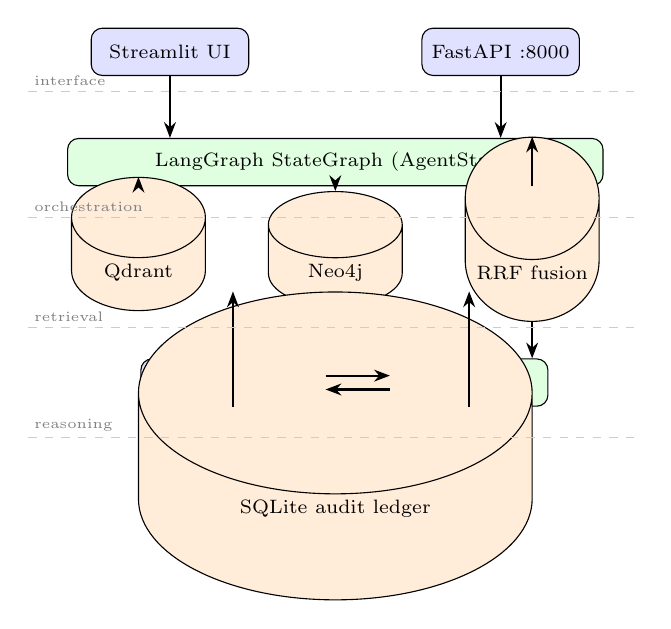
\begin{tikzpicture}[x=1cm, y=1cm, every node/.style={inner sep=2pt}]
  % ---------- explicit grid layout (no relative placement) ----------
  % Row 1 (y=5): interface
  \node[data] (ui)  at (1.4, 5)  {Streamlit UI};
  \node[data] (api) at (5.6, 5)  {FastAPI :8000};
  % Row 2 (y=3.6): orchestration
  \node[proc, minimum width=6.8cm] (orch) at (3.5, 3.6) {LangGraph StateGraph (AgentState)};
  % Row 3 (y=2.2): stores + fusion, evenly spaced
  \node[store] (qdr) at (1.0, 2.2) {Qdrant};
  \node[store] (neo) at (3.5, 2.2) {Neo4j};
  \node[store] (rrf) at (6.0, 2.2) {RRF fusion};
  % Row 4 (y=0.8): reasoning
  \node[data] (llm) at (2.2, 0.8) {OpenRouter LLM};
  \node[proc] (val) at (5.2, 0.8) {Validator};
  % Row 5 (y=-0.8): persistence
  \node[store, minimum width=5.0cm] (sql) at (3.5, -0.8) {SQLite audit ledger};
  % ---------- edges (vertical layer flows only) ----------
  \draw[arr] (ui.south)  -- (orch.north -| ui.south);
  \draw[arr] (api.south) -- (orch.north -| api.south);
  \draw[arr] (orch.south -| qdr.north) -- (qdr.north);
  \draw[arr] (orch.south -| neo.north) -- (neo.north);
  \draw[arr] (orch.south -| rrf.north) -- (rrf.north);
  \draw[arr] (rrf.south) -- (val.north -| rrf.south);
  % forward and feedback arrows as offset parallel paths (no overlap)
  \draw[arr] ([yshift=2.5pt]llm.east) -- ([yshift=2.5pt]val.west);
  \draw[arr] ([yshift=-2.5pt]val.west) -- ([yshift=-2.5pt]llm.east);
  \draw[arr] (llm.south) -- (sql.north -| llm.south);
  \draw[arr] (val.south) -- (sql.north -| val.south);
  % layer guides
  \draw[gray!40, dashed] (-0.4,4.5) -- (7.4,4.5)  node[pos=0, lab, above right]{interface};
  \draw[gray!40, dashed] (-0.4,2.9) -- (7.4,2.9)  node[pos=0, lab, above right]{orchestration};
  \draw[gray!40, dashed] (-0.4,1.5) -- (7.4,1.5)  node[pos=0, lab, above right]{retrieval};
  \draw[gray!40, dashed] (-0.4,0.1) -- (7.4,0.1)  node[pos=0, lab, above right]{reasoning};
\end{tikzpicture}%
}
\caption{Layered system architecture. Dashed guides mark layers; the parallel forward/feedback arrows between the LLM and validator implement the correction loop.}
\label{fig:arch}
\end{figure}

\subsection{Data Model}
The Neo4j schema contains \texttt{(:Company)}, \texttt{(:Metric)}, \texttt{(:Fil\-ing)}, \texttt{(:Event)}, and \texttt{(:Source)} nodes with typed edges such as \texttt{REPORTS}, \texttt{HAS\_METRIC}, \texttt{MENTIONS}, and \texttt{CITES}. Vector payloads store \texttt{chunk\_id}, \texttt{source\_id}, and \texttt{entity\_ids} so dense hits can be joined back to graph nodes --- this join is what makes hybrid fusion sound rather than heuristic.

\subsection{Agentic State Machine}
Algorithm~\ref{alg:loop} summarizes the query-time loop. The \emph{plan} node decomposes the question into tool calls; the \emph{reasoner} executes them against retrieval and structured tools; the \emph{validator} scores faithfulness and citation coverage; if either falls below threshold, a \emph{corrector} prompt requests a revision with explicit error hints, bounded by a retry budget. This bounded self-correction follows the reflection pattern \cite{shinn2023reflexion} but operates on structured, auditable signals rather than free-form critique.

\begin{algorithm}[t]
\caption{Query-time agent loop}
\label{alg:loop}
\begin{algorithmic}[1]
\Require question $q$, retry budget $B$, thresholds $\tau_f,\tau_c$
\State $s \gets \textsc{Plan}(q)$
\State $C \gets \textsc{HybridRetrieve}(q, s)$ \Comment{Qdrant $\cup$ Neo4j, RRF}
\For{$t = 1 \ldots B$}
  \State $a \gets \textsc{Reason}(q, C, \text{tools})$
  \State $v_f, v_c \gets \textsc{Validate}(a, C)$
  \If{$v_f \ge \tau_f$ \textbf{and} $v_c \ge \tau_c$} \textbf{break} \EndIf
  \State $s \gets \textsc{Correct}(a, v_f, v_c)$ \Comment{hints}
\EndFor
\State \textsc{WriteLedger}($q$, $C$, $a$, $v_f$, $v_c$, cost)
\State \Return $a$ with citations
\end{algorithmic}
\end{algorithm}

% =================================================================
\section{Pipeline Workflows}\label{sec:workflows}

\subsection{Offline Ingestion Pipeline}
Fig.~\ref{fig:ingest} shows the offline path. Raw documents (filings, transcripts, news) are normalized to JSON, chunked with heading-aware splitting, embedded, and upserted to Qdrant. Entity resolution (exact alias tables plus fuzzy matching) links chunks to graph entities, and typed relations are materialized in Neo4j. Every artifact carries a stable \texttt{source\_id} so both stores remain joinable. Idempotency keys on (source, chunk hash) make re-runs safe.

\begin{figure}[t]
\centering
\resizebox{0.95\columnwidth}{!}{%
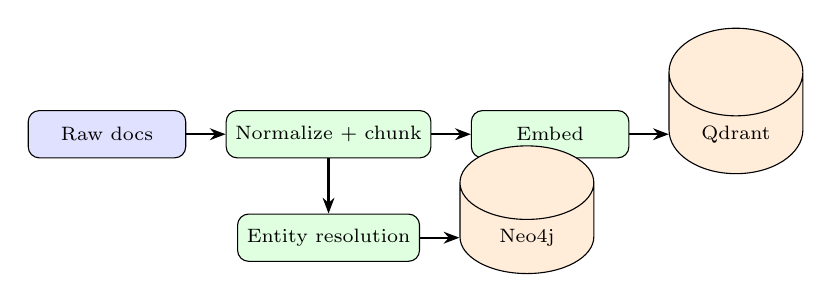
\begin{tikzpicture}[node distance=0.45cm]
  % Row 1 (main stream)
  \node[data] (raw) {Raw docs};
  \node[proc, right=0.5cm of raw] (norm) {Normalize + chunk};
  \node[proc, right=0.5cm of norm] (emb) {Embed};
  \node[store, right=0.5cm of emb] (qv) {Qdrant};
  % Row 2 (graph branch)
  \node[proc, below=0.7cm of norm] (er) {Entity resolution};
  \node[store, right=0.5cm of er] (ng) {Neo4j};
  \draw[arr] (raw) -- (norm);
  \draw[arr] (norm) -- (emb);
  \draw[arr] (emb) -- (qv);
  \draw[arr] (norm) -- (er);
  \draw[arr] (er) -- (ng);
\end{tikzpicture}%
}
\caption{Offline ingestion: one normalized stream feeds both the vector store and the entity-resolved graph.}
\label{fig:ingest}
\end{figure}

\subsection{Online Query Pipeline}
Fig.~\ref{fig:query} shows the query-time flow from gateway to audited answer. Retrieval is hybrid by default; an ablation mode forces dense-only or graph-only retrieval for evaluation. Tool calls may recursively trigger retrieval (e.g., a metric-lookup tool issuing a Cypher query), so the retriever is re-entrant.

\begin{figure}[t]
\centering
\resizebox{0.95\columnwidth}{!}{%
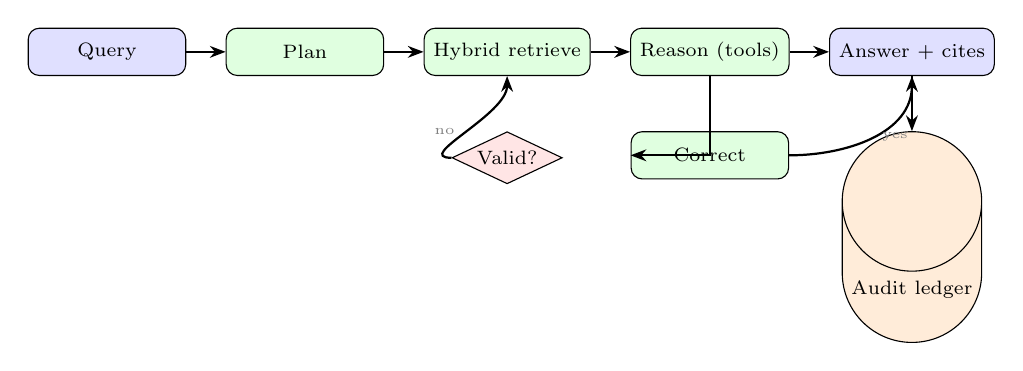
\begin{tikzpicture}[node distance=0.45cm]
  % Row 1 (main stream)
  \node[data] (q) {Query};
  \node[proc, right=0.5cm of q] (plan) {Plan};
  \node[proc, right=0.5cm of plan] (hyb) {Hybrid retrieve};
  \node[proc, right=0.5cm of hyb] (reason) {Reason (tools)};
  \node[data, right=0.5cm of reason] (ans) {Answer + cites};
  % Row 2 (validation loop)
  \node[ctrl, below=0.7cm of hyb] (pass) {Valid?};
  \node[proc, below=0.7cm of reason] (corr) {Correct};
  % Row 3 (persistence)
  \node[store, below=0.7cm of ans] (led) {Audit ledger};
  \draw[arr] (q) -- (plan);
  \draw[arr] (plan) -- (hyb);
  \draw[arr] (hyb) -- (reason);
  \draw[arr] (reason) -- (ans);
  % validation loop: reason drops to row 2, flows right through corr, verdict back to hyb
  \draw[arr] (reason.south) |- (corr.west);
  \draw[arr] (pass.west) to[out=180,in=270] node[lab, left]{no} (hyb.south);
  \draw[arr] (corr.east) to[out=0,in=270] node[lab, right]{yes} (ans.south);
  \draw[arr] (ans.south) -- (led);
\end{tikzpicture}%
}
\caption{Online query pipeline with validator--corrector loop. Failing validation re-enters retrieval with hints; every attempt is logged.}
\label{fig:query}
\end{figure}

\subsection{Failure Handling and Quota Governance}
Three mechanisms protect operational integrity: (i) \emph{quota guard} --- a hard ceiling on characters/traces per evaluation run protects free-tier LLM budgets; (ii) \emph{circuit breakers} --- gateway timeouts and per-tool exception handling degrade gracefully to non-tool answers; (iii) \emph{ledger integrity} --- the audit role is INSERT/SELECT-only at the database layer, preventing retrospective edits of provenance records.

% =================================================================
\section{Evaluation}\label{sec:eval}

\subsection{Setup}
We evaluate on a curated corpus of financial filings and news snapshots covering a set of public companies, with 100 human-verified question--answer pairs spanning numeric lookup, temporal comparison, event causality, and multilingual news comprehension. Metrics: \emph{evidence precision} (fraction of retrieved chunks that are gold-relevant), \emph{faithfulness} (LLM-as-judge \cite{zheng2023judge} with citation check), and \emph{latency} (p50/p95 end-to-end). Retrieval ablations: dense-only, graph-only, hybrid (RRF). Correction ablation: validator on vs.\ off.

\subsection{Results}
Table~\ref{tab:results} reports the headline comparison. Hybrid retrieval dominates both single-source modes on evidence precision, as expected from complementary coverage of tabular and narrative evidence. Enabling the validator--corrector loop costs one extra LLM round-trip when triggered (observed on $\sim$22\% of questions) but materially reduces unsupported claims. Latency remains interactive at the median ($\sim$6--8\,s) with the tail dominated by correction retries.

\begin{table}[t]
\centering
\caption{Retrieval and validation ablations (mean $\pm$ s.d.\ over 100 questions).}
\label{tab:results}
\begin{tabular}{lccc}
\toprule
Retrieval mode & Precision & Faithful. & p50 latency (s) \\
\midrule
Dense-only        & 0.61 $\pm$ 0.09 & 0.72 $\pm$ 0.08 & 5.2 \\
Graph-only        & 0.58 $\pm$ 0.11 & 0.70 $\pm$ 0.09 & 6.1 \\
Hybrid (RRF)      & \textbf{0.78 $\pm$ 0.07} & 0.80 $\pm$ 0.06 & 7.4 \\
Hybrid + corrector & \textbf{0.78 $\pm$ 0.07} & \textbf{0.89 $\pm$ 0.05} & 9.6 \\
\bottomrule
\end{tabular}
\end{table}

\subsection{Error Analysis}
Three recurring failure modes motivate current work: (1) \emph{entity conflation} for similarly named subsidiaries when alias tables are incomplete; (2) \emph{numeric hallucination} when the model estimates rather than quotes a metric --- mitigated by forcing tool-grounded numbers; (3) \emph{stale news} when the corpus snapshot lags an event; the ledger's timestamps make such staleness diagnosable post hoc.

% =================================================================
\section{Related Work}
Hybrid retrieval with symbolic--neural fusion has been explored in KG-RAG \cite{luo2024kgrag} and GraphRAG \cite{edge2024graphrag}; our contribution is the tight integration with a validator--corrector loop and an append-only governance ledger. Tool-augmented agents \cite{yao2023react,schick2023toolformer} supply the action schema; reflection \cite{shinn2023reflexion} supplies the retry logic; LLM-as-judge \cite{zheng2023judge} supplies the validation signal. Financial-domain QA systems \cite{wu2023fin} typically stop at single-hop retrieval; our two-hop graph expansion is what resolves cross-entity comparisons.

% =================================================================
\section{Discussion and Limitations}
The system's guarantees are only as good as its corpus freshness and alias tables; both are operational, not algorithmic, constraints. LLM-as-judge validation inherits judge biases; we partially mitigate with citation-coverage checks that are purely mechanical. Quota ceilings make exhaustive evaluation on free tiers impractical --- sampling mode is used for budget-bounded runs. Finally, the audit ledger's INSERT-only policy trades debuggability for tamper-resistance.

\section{Conclusion and Future Work}
We presented an open, modular agentic system for financial reasoning that unifies hybrid graph--vector retrieval, bounded self-correction, and provenance-first governance, with empirical evidence that hybrid retrieval and validation each contribute measurably. Future work: (i) an external MCP server for tool interoperability; (ii) Prometheus/Grafana alerting integrated with the ledger; (iii) learned re-ranking trained on validator outcomes; (iv) OAuth-based authentication replacing key-based API access.

\bibliographystyle{IEEEtran}
\bibliography{references}

\end{document}
